\section{Theoretical Background in Reinforcement Learning}
Reinforcement learning is an approach in artificial intelligence for goal-directed learning from interaction and experience, that makes it different from the other approaches in machine learning in which the learner, the decision maker, or the so called agent, is told what to do. In reinforcement learning the agent tries out different actions in order to understand which of them generates the most reward. The reward is a special term in reinforcement learning which describes the goal in a Markov decision process (MDP) model. Roughly speaking, the MDP model would very well characterize the agent’s view of the world, the actions that it can take in the world and its goal.

Machine learning distinguishes supervised from unsupervised learning paradigms by having the supervisor indicating the correct behavior in certain generalized situations for the supervised learning and finding hidden structure in unlabeled data for the unsupervised learning. Reinforcement learning is sometimes classified as an unsupervised learning problem, because it doesn’t make use of labeled data, however it doesn’t look for structure, but tries to maximize the reward. Therefore, reinforcement learning is considered another paradigm in machine learning, according to the opinion and points of the authors R. S. Sutton and A. G. Barto of the book “An introduction to Reinforcement Learning” \cite{Sutton}. The diagram in \Cref{fig:RLandML} illustrates the relationship between machine learning and reinforcement learning.
\begin{figure}[H]
	\centering
	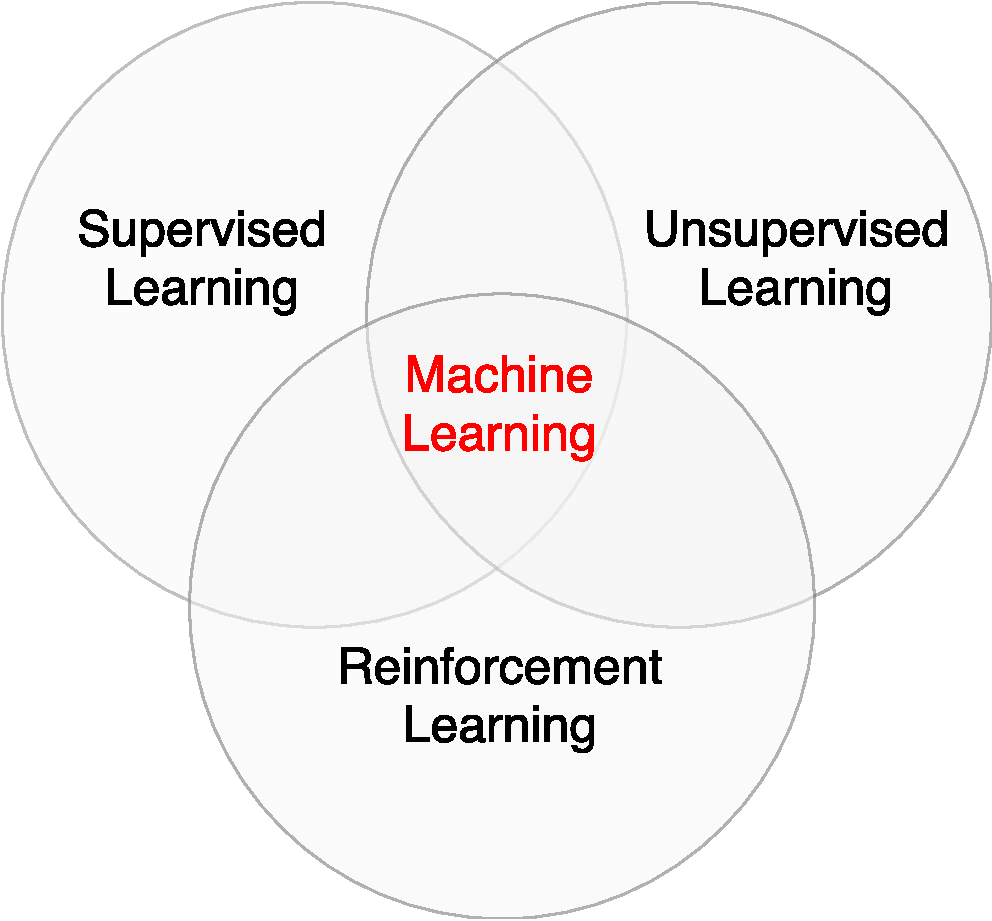
\includegraphics[width=0.7\textwidth]{Figures/RLandML}
	\caption{Reinforcement Learning and Machine Learning}
	\label{fig:RLandML}
\end{figure}
Reinforcement learning considers the problem of planning in real time decision making and the models for prediction related to planning. The interactive goal-directed agent is able to operate in an uncertain set up, make decisions despite uncertainty and predict future events. The agent is not necessarily a robot; it can be any component in a larger system in which it interacts directly with the system and indirectly with the system’s environment. The environment is everything that the agent interacts with, it is the outer world.

There is a special concern in reinforcement learning which is not present in the other machine learning approaches. It is the issue of balancing exploitation of the knowledge that the agent has and exploration of new information in order to improve the current knowledge base.

A variety of different scientific fields intersect with reinforcement learning, especially mathematics, namely, statistics and optimization, which have an important background contribution to the reinforcement learning methods. “For example, the ability of some reinforcement learning methods to learn with parameterized approximators addresses the classical “curse of dimensionality” in operations research and control theory.” \cite{Sutton} The relationship between reinforcement learning and optimization can be exemplified by the idea of maximization of the reward signal. Actually, in reinforcement learning the agent intends to maximize the reward, but not necessarily achieves the maximum. Reinforcement learning is also part of the engineering and computer science subjects. The related algorithms have a close resemblance to the biological brain systems of animals and humans due to the reward factor involved, therefore it also binds with the psychology and neuroscience fields. The diagram in \Cref{fig:RLandOther} illustrates how reinforcement learning relates to other scientific disciplines.
\begin{figure}[H]
	\centering
	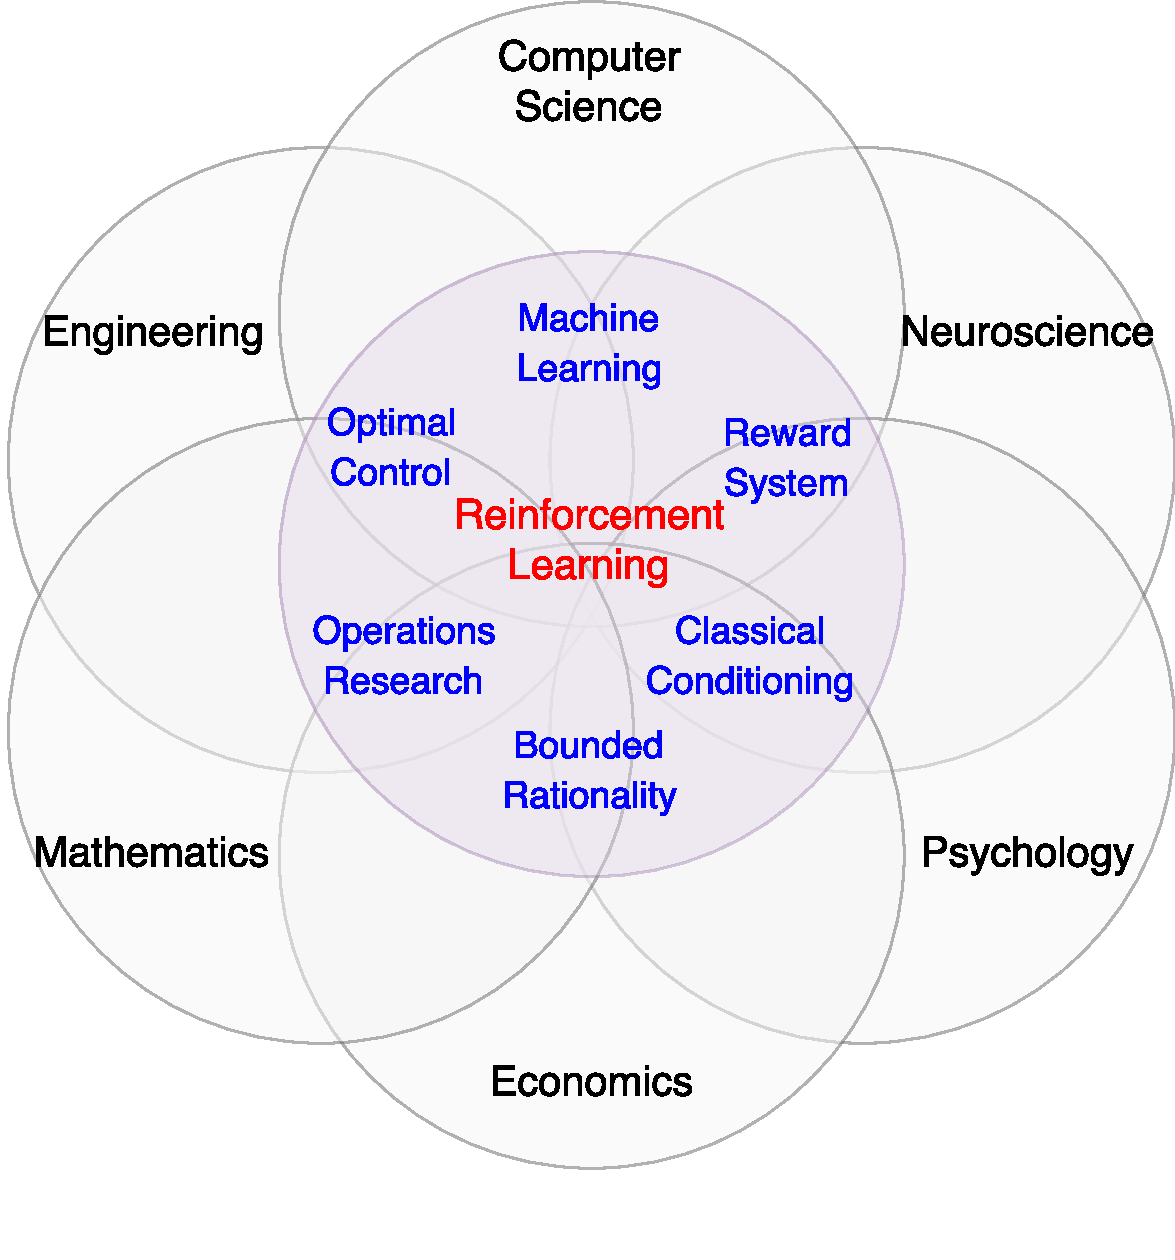
\includegraphics[width=0.7\textwidth]{Figures/RLandOther}
	\caption{Reinforcement Learning and other disciplines}
	\label{fig:RLandOther}
\end{figure}
\subsection{Elements of a reinforcement learning problem}
A reinforcement learning problem contains at least one of the elements: reward signal, value function, policy, environment model.

The reward signal represents a feedback from the environment as a response to the agent’s behavior in that environment, therefore the agent cannot change the feedback that it receives, but it can behave accordingly so as to maximize the gained reward signals during its lifetime. The “reward signal defines the goal in a reinforcement learning problem” \cite{Sutton}. It serves as a problem definition and as a basis for modifying the policy.

The policy maps states to actions, so that when the agent is in a specific state, it chooses an action based on the defined policy. A policy is enough to describe the behavior of the agent and therefore, it is the core of reinforcement learning.

The value function provides values for judging about the quality of a state based on the estimated maximum reward it can yield in the long run, in contrast with the reward which expresses only the immediate advantage of being in a specific state.

The model is a representation of the environment’s behavior. In a model-free reinforcement learning (trial-and-error) problem the agent cannot plan its future, because it doesn’t have a model basis, whereas in mode-based problems the agent can plan its future actions based on the environment’s modelled behavior and expected rewards in certain states.
\subsection{Solution methods}
The solution methods for the reinforcement learning problem can be divided into two groups, tabular and approximate. The tabular solution methods find exact, optimal solutions and are more suitable when the states and actions space is rather small, while the approximate solution methods provide approximate solutions and it is applicable to large spaces problems.

The tabular solution methods include three important classes of methods for solving the finite MDP: dynamic programming, Monte Carlo and temporal-difference learning. Combinations of these and addition of other features like eligibility traces, model learning would result in better approaches.

The approximate solution methods are an extension to the tabular solution methods for huge states spaces problems. In these type of problems, the goal is to find a good approximate solution under the condition of restricted computational resources. Because almost every visited state is seen for the first time, every state being so unique, the agent needs to be able to make sense of it and, therefore, usefully generalize the information it gets. This is possible thanks to function approximation. “Function approximation is an instance of supervised learning, the primary topic studied in machine learning, artificial neural networks, pattern recognition, and statistical curve fitting” \cite{Sutton}.
\subsection{Markov Decision Processes for Reinforcement Learning}
The general reinforcement learning problem formulation has the format of a finite MDP. The interaction between the agent and environment happens at each time step of a sequence of discrete time steps, $t=0,1,2,3,...$, where at each time step $t$ the agent receives a representation of the world - a state, $S_{t}\epsilon S$, from a set of possible states $S$, selects an action $A_{t}$ from a set of possible actions $A(S_{t})$ for the state $S_{t}$ by implementing a policy $\pi_{t}$, where $\pi_{t}(a|s)$ is the probability that $A_{t}=a$ if $S_{t}=s$, and in the next time step $t+1$ the agent receives a reward signal $R_{t+1}\epsilon R$ from the environment ending up in a new state $S_{t+1}$ \cite{Sutton}. The diagram in \Cref{fig:AgentEnv} illustrates the interaction between the agent and the environment.
\begin{figure}[H]
	\centering
	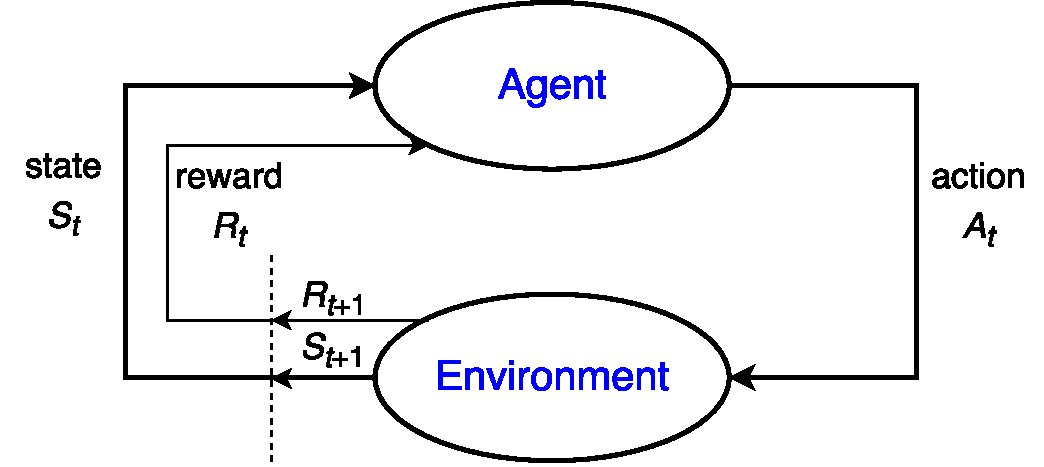
\includegraphics[width=0.7\textwidth]{Figures/Agent-EnvironmentInteraction}
	\caption{Agent - environment interaction}
	\label{fig:AgentEnv}
\end{figure}
Reinforcement learning methods provide ways to adjust the policy based on the accumulated experience with the goal of maximizing the total cumulative reward in mind. An example for representing the goal in a reinforcement learning problem like that of making a robot learn to walk would be by giving a reward on each time step proportional to the robot's forward motion. “The reward signal is your way of communicating to the robot what you want it to achieve, not how you want it achieved” \cite{Sutton}.

A formal definition of the cumulative reward received in the long run is expressed by the expected return $G_{t}$ which is a function of rewards sequence $R_{t+1},R_{t+2},...,R_{T}$ received after the time step $t$, where $T$ is the last time step:\begin{equation}
G_{t}=R_{t+1}+R_{t+2}+...+R_{T}
\end{equation}
This is the case for the episodic tasks where there is a terminal state after some time steps. But there might be cases in which the process is continuous and the final step is infinite, therefore the return could also be infinite. In order to express the return more conveniently the concept of discounting is introduced which determines the current value of the future rewards:

formula 
where the discount rate is between 0 and 1.

With the discounting factor, the reward received after $k$ time steps has the value discount rate power k-1 times what it would be worth if it were received immediately. This makes the return have a finite value, under the condition that the reward sequence is finite. In the extreme point of discount = 0, it is said that the agent is myopic because it only maximizes over the immediate rewards and not the future rewards, whereas if the discount is closer to 1 the agent is farsighted and sees far into the future considering the future rewards when picking actions.